% !TEX TS-program = pdflatex
% !TEX encoding = UTF-8 Unicode

% This is a simple template for a LaTeX document using the "article" class.
% See "book", "report", "letter" for other types of document.

\documentclass[10pt]{article} % use larger type; default would be 10pt

\usepackage[utf8]{inputenc} % set input encoding (not needed with XeLaTeX)

%%% Examples of Article customizations
% These packages are optional, depending whether you want the features they provide.
% See the LaTeX Companion or other references for full information.

%%% PAGE DIMENSIONS
\usepackage{geometry} % to change the page dimensions
\geometry{letterpaper} % or letterpaper (US) or a5paper or....
\geometry{margin=1in} % for example, change the margins to 2 inches all round
% \geometry{landscape} % set up the page for landscape
%   read geometry.pdf for detailed page layout information

\usepackage{graphicx} % support the \includegraphics command and options
\usepackage{mathrsfs}
% \usepackage[parfill]{parskip} % Activate to begin paragraphs with an empty line rather than an indent

%%% PACKAGES
\usepackage{booktabs} % for much better looking tables
\usepackage{array} % for better arrays (eg matrices) in maths
\usepackage{paralist} % very flexible & customisable lists (eg. enumerate/itemize, etc.)
\usepackage{verbatim} % adds environment for commenting out blocks of text & for better verbatim
\usepackage{subfig} % make it possible to include more than one captioned figure/table in a single float
\usepackage[font=small,labelfont=bf]{caption} % Required for specifying captions to tables and figures
% These packages are all incorporated in the memoir class to one degree or another...

%%% HEADERS & FOOTERS
\usepackage{fancyhdr} % This should be set AFTER setting up the page geometry
\pagestyle{fancy} % options: empty , plain , fancy
\renewcommand{\headrulewidth}{0pt} % customise the layout...
\lhead{}\chead{}\rhead{}
\lfoot{}\cfoot{\thepage}\rfoot{}

%%% SECTION TITLE APPEARANCE
\usepackage{sectsty}
\allsectionsfont{\sffamily\mdseries\upshape} % (See the fntguide.pdf for font help)
% (This matches ConTeXt defaults)

%%% ToC (table of contents) APPEARANCE
\usepackage[nottoc,notlof,notlot]{tocbibind} % Put the bibliography in the ToC
\usepackage[titles,subfigure]{tocloft} % Alter the style of the Table of Contents
\renewcommand{\cftsecfont}{\rmfamily\mdseries\upshape}
\renewcommand{\cftsecpagefont}{\rmfamily\mdseries\upshape} % No bold!
\newcommand{\centerfig}[2]{\begin{center}\includegraphics[width=#1\textwidth]{#2}\end{center}}
\usepackage{amssymb}
\usepackage{mathtools}
\DeclarePairedDelimiter\ceil{\lceil}{\rceil}
\DeclarePairedDelimiter\floor{\lfloor}{\rfloor}
\let\oldemptyset\emptyset
\let\emptyset\varnothing
\usepackage[usenames, dvipsnames]{color}
\makeatletter
\def\@maketitle{%
  \newpage
  \null
  \vskip 1em%
  \begin{center}%
  \let \footnote \thanks
	\vskip -5em%
    {\LARGE \@title \par}%
    \vskip 1em
    {\large
      \lineskip .5em%
      \begin{tabular}[t]{c}%
        \@author
      \end{tabular}\par}%
    \vskip 1em%
    {\large \@date}%
  \end{center}%
  \par
  \vskip 1.5em}
\makeatother
%%% END Article customizations

%%% The "real" document content comes below...

\title{Physics 410: Project 1}
\author{Arnold Choa -- 32038144}
\date{10 October, 2018} % Activate to display a given date or no date (if empty),
         % otherwise the current date is printed 
%{\color{red}{\normalsize{\textbf{TODO}}}} %TODO signage
\begin{document}
\maketitle
\vspace{-0.5cm}
\noindent \Large{Execise 2.16}
\\ \\
\normalsize{For this exercise, I will first give a refresher on the Single Quantum Well System (both finite and infinite variants). I will then talk about what the propagator method yields and how to derive it and its properties. Finally, I will compare the solution we get using the propagator method with the analytical solutions for the quantum square well and show them to be exactly the same.}
\\ \\
\noindent As a starting point, we can write Schr{\"o}dinger's famous wave equation and the potential for a square well:
\begin{equation}
-\frac{\hbar ^{2}}{2m}\frac{d^2 \Psi}{dx^2} + V(x)\Psi (x) = E \Psi (x)
\end{equation}
\begin{equation}
V(x) = 
\begin{cases}
	0 ; b\leq x \leq c \\
	V_{0};\ otherwise
\end{cases}
\end{equation}
\noindent For an infinite square well, let $V_{0} = \infty$. For now, let $b = -a$ and $c = a$. Looking at our well, we can split the space into 3 distinct regions: the left of the well (I), the well itself (II), and the right of the well (III).
\centerfig{.3}{../figs/single_well.png}
\captionof{figure}{Square well Potential. Region I, II, and III are respectively shown.}
For a square well, we know that the general solutions for regions I, II, and III are as follows:
\begin{equation}
\Psi (x) = 
\begin{cases}
	Ce^{\beta x}; x\ in\ I\\
	A\sin (\alpha x) + B\cos (\alpha x); x\ in\ II\\
	Fe^{ - \beta x}; x\ in\ III
\end{cases}
\end{equation}
where $\alpha = \sqrt{\frac{2mE}{\hbar ^{2}}}$ and $\beta = \sqrt{2m(V_{0} - E) / \hbar ^2}$. As $V_{0} \rightarrow \infty$, $\Psi_I = \Psi_I' = \Psi_{II} = \Psi_{II}' = 0$ leading  to the infinite square well solution.

\noindent To find the allowed energy levels, we note that we need continuity and differentiability at I-II and II-III. so:
\begin{equation}
at\ x=-a:
\begin{cases}
-A\sin (\alpha a) + B\cos (\alpha a) = Ce^{-\beta a} \\
\alpha A\alpha \cos (\alpha a) + \alpha B\sin (\alpha a) = \beta Ce^{-\beta a} \\
\end{cases}
\end{equation}
\begin{equation}
at\ x=a:
\begin{cases}
A\sin (\alpha a) + B\cos (\alpha a) = Fe^{-\beta a} \\
\alpha A\alpha \cos (\alpha a) - \alpha B\sin (\alpha a) = -\beta Fe^{-\beta a} \\
\end{cases}
\end{equation}
\noindent For infinite $V_0$, since the RHS for the top equations of each bracket must be identically 0, this leads to $E_n = \frac{(n + 1/2)^2 \pi ^2 \hbar^2}{2ma^2}, n = 0,1,\dots$ and $E_n = \frac{(n)^2 \pi ^2 \hbar^2}{2ma^2}, n = 1,2,\dots$ for the even and odd solutions respectively.
\\ \\
\noindent For finite $V_0$, we can solve for the energy levels by looking for the roots for $\alpha \tan(\alpha a) = \beta$ and $\alpha \cot(\alpha a) = -\beta$ from the even and odd states respectively.
\newpage
\noindent Moving on to the propagator method, we observe that for a finite (or even infinite well), the solutions for Region II as above (now we do not need to restrict ourselves to the symmetric case) have the form:
\begin{equation}
\Psi _{II}(x) = A\sin (\alpha x) + B\cos (\alpha x); b\leq x \leq c
\end{equation}
\begin{equation}
\Psi _{II}'(x) = \alpha A\cos (\alpha x) - \alpha  B\sin (\alpha x); b\leq x \leq c
\end{equation}
where $b$ and $c$ are the positions of the left and right wall of the well. $\alpha$ is to be determined by the boundary conditions. Assuming we know $\Psi (b)$ and $\Psi ' (b)$, by the question, we can isolate $A$ and $B$:
\begin{equation}
A = \sin(\alpha b)\Psi (b) + \frac{1}{\alpha}\cos (\alpha b) \Psi ' (b)
\end{equation}
\begin{equation}
B = \cos(\alpha b)\Psi (b) - \frac{1}{\alpha}\sin (\alpha b) \Psi ' (b)
\end{equation}
\noindent Now that we have $A$ and $B$, we replug these coefficients into (6) and (7) yielding:
\begin{align}
	\Psi _{II}(x) 	&= A\sin (\alpha x) + B\cos (\alpha x)\\
			&= \left(\sin(\alpha b)\Psi (b) + \frac{1}{\alpha}\cos (\alpha b) \Psi ' (b)\right) \sin (\alpha x) + \left(\cos(\alpha b)\Psi (b) - \frac{1}{\alpha}\sin (\alpha b) \Psi ' (b)\right)\cos (\alpha x)\\
			&= \left( \sin(\alpha b)\sin(\alpha x) + \cos(\alpha b)\cos(\alpha x) \right) \Psi(b) + \frac{1}{\alpha} \left(\cos(\alpha b)\sin(\alpha x) - \sin(\alpha b)\cos(\alpha x) \right) \Psi ' (b)\\
			&= \cos(\alpha(x - b))\Psi(b) + \frac{1}{\alpha}\sin(\alpha(x-b))\Psi'(b)
\end{align}
\begin{align}
	\Psi' _{II}(x) 	&= \alpha \left( A\cos (\alpha x) -  B\sin (\alpha x) \right)\\
			&= \alpha \left( \left(\sin(\alpha b)\Psi (b) + \frac{1}{\alpha}\cos (\alpha b) \Psi ' (b)\right)\cos (\alpha x) - \left(\cos(\alpha b)\Psi (b) - \frac{1}{\alpha}\sin (\alpha b) \Psi ' (b)\right)\sin (\alpha x) \right)\\
			&= \alpha(\sin(\alpha b)\cos(\alpha x) - \cos(\alpha b)\sin(\alpha x))\Psi(b) + (\cos(\alpha b)\cos(\alpha x) + \sin(\alpha b)\sin(\alpha x))\Psi ' (b)\\
			&= -\alpha(\sin(\alpha(x-b)))\Psi(b) + \cos(\alpha (x-b))\Psi'(b)
\end{align}
\noindent We can re-write these equations in vector-mmatrix notation:
\begin{equation}
\left[ \begin{array}{c} \Psi(x) \\ \Psi'(x)\end{array}\right] = P_{allowed} \left[ \begin{array}{c} \Psi(b) \\ \Psi'(b)\end{array}\right]
\end{equation}
\begin{equation}
P_{allowed} = \left[ \begin{array}{c c} \cos(\alpha(x-b)) & \frac{1}{\alpha}\sin(\alpha(x-b)) \\ -\alpha(\sin(\alpha(x-b))) & \cos(\alpha(x-b))\end{array}\right]
\end{equation}
\noindent With Eq. 18 and 19, we can know propagate our wavefunction within the square well. As for what $\alpha$ we need, we can deduce those from our continuity conditions.
\\ \\
\noindent We note that the solutions for Regions I and III have the form:
\begin{equation}
\Psi (x) = 
\begin{cases}
	Ce^{\beta x}; x \leq b\\
	Fe^{ - \beta x}; x \geq c
\end{cases}
\end{equation}
\begin{equation}
\Psi' (x) = 
\begin{cases}
	\beta Ce^{\beta x}; x \leq b\\
	-\beta Fe^{ - \beta x}; x\geq c
\end{cases}
=
\begin{cases}
	\beta \Psi(x); x \leq b\\
	-\beta \Psi(x); x\geq c
\end{cases}
\end{equation}
\noindent where as in the square well, $\alpha = \sqrt{\frac{2mE}{\hbar ^{2}}}$ and $\beta = \sqrt{2m(V_{0} - E) / \hbar ^2}$. By continuity constraints, $\Psi' (b) = \beta\Psi(b)$ and  $\Psi' (c) = -\beta\Psi(c)$. If we know $\Psi (b)$, we can figure out $\Psi' (b)$, use the propagation method from Eq. 18, and learn $\Psi (c)$ and $\Psi'(c)$, and then $\beta$, $\alpha$, and subsequently $E$.
\newpage
\noindent Now, let us compare the eigenvalues  we get via the propagator method and the analytical solution.
\\ \\ First we note that part of the propagator method breaks down at the infinite square well. Because of continuity constraints, if we strictly followed our train of thought here, we would only get $\left[ \begin{array}{c} \Psi(b) \\ \Psi'(b)\end{array}\right] =\left[ \begin{array}{c} 0 \\ 0\end{array}\right]$ if we solely based it on $\Psi (b)$. We would then have to observe $\Psi' (b)$ as well, and get a non-zero value here, to not get a trivial propagation. We thus note that $\Psi(c) = 0$ and we can now solve $\alpha$ based on the propagation.  In this  case, we need $\sin(\alpha (c-b))= 0; \alpha \neq 0$. Thus, $\alpha = \frac{k \pi}{(c-b)}$ leading to $\frac{n\pi}{(c-b)} = \sqrt{\frac{2mE}{\hbar ^{2}}}$. Re-writing to a more suggestive form:
\begin{equation}
	E_{n} = \frac{\left(\frac{n}{2}\right)^2 \pi^2 \hbar^2}{2m\left(\frac{c-b}{2}\right)^2}
\end{equation}
\noindent which holds the eigenvalues for both the even and odd states (let n = 2k and n = 2k+1). We have thus shown the two methods to be equivalent for the infinite square well case.
\\ \\
We will now look into the finite square well case. Given that $\Psi(b) = a, a \neq 0$, by using continuity constraints, we know that:
\begin{equation}
\Psi'(b) = \beta \Psi(b) = \beta a; x = b
\end{equation}
\begin{equation}
\Psi'(c) = -\beta \Psi(c); x = c
\end{equation}
\noindent This is also true for Region II, thus, we can rewrite all the functions in terms of Region II leading to:
\begin{align}
\Psi'(b) 	&= \beta \left(\cos(\alpha(b - b))\Psi(b) + \frac{1}{\alpha}\sin(\alpha(b-b))\Psi'(b)\right)\\
		&= \beta \Psi(b)
\end{align}
\begin{equation}
-\alpha(\sin(\alpha(c-b)))\Psi(b) + \cos(\alpha (c-b))\Psi'(b) = -\beta\left( \cos(\alpha(c - b))\Psi(b) + \frac{1}{\alpha}\sin(\alpha(c-b))\Psi'(b) \right)
\end{equation}
\begin{equation}
-\alpha(\sin(\alpha(c-b)))\Psi(b) + \cos(\alpha (c-b))\beta \Psi(b) = -\beta\left( \cos(\alpha(c - b))\Psi(b) + \frac{\beta}{\alpha}\sin(\alpha(c-b))\Psi(b) \right)
\end{equation}
We let $x = \alpha\frac{c-b}{2}$:
\begin{align}
0	&=  \Psi(b) \left[ \frac{\beta^2 - \alpha^2}{\alpha}\sin(2x)  + 2\beta\cos(2x)\right]\\
	&=  2\Psi(b) \left[ \frac{\beta^2 - \alpha^2}{\alpha}\sin(x)\cos(x)  + \beta\cos^2(x) - \beta\sin^2(x)\right]\\
	&=  2\Psi(b) \left[ \left(\beta^2 - \alpha^2\right)\sin(x)\cos(x)  + \alpha\beta\cos^2(x) - \alpha\beta\sin^2(x)\right]\\
	&= 2\Psi(b)\left[ \alpha\cos(x)\left( \beta\cos(x) - \alpha\sin(x) \right) + \beta\sin(x)\left( \beta\cos(x) - \alpha\sin(x) \right) \right]\\	
	&=  2\Psi(b) \left[ \beta\cos(x) - \alpha\sin(x)\right] \left[ \beta\sin(x) + \alpha\cos(x)\right]
\end{align}
Since $\Psi(b) \neq 0$ our roots will either come from:
\begin{equation}
\alpha \sin\left(\alpha \frac{c-b}{2} \right) = \beta\cos\left(\alpha \frac{c-b}{2} \right)
\end{equation}
\begin{equation}
\alpha \cos\left(\alpha \frac{c-b}{2} \right) = - \beta \sin\left(\alpha \frac{c-b}{2} \right)
\end{equation}
giving us our original formulae for our eigenvalues.
\newpage
\noindent \Large{Exercise 2.18}
\\ \\
\normalsize{Please see \textit{q2\_18.py} in the code folder for relevant code for this exercise}
\\ \\
\noindent Given the specifications based on the problem, we learned that the eigenvalues for the system are at $E(in\ eV) = \{0.704880, 0.725492, 2.770146, 2.871760, 6.000818, 6.318130, 9.775956\}$.
\\ \\
\noindent We also plotted the two lowest energies as a function of separation distance. What we notice is that these energies are perceived to be steps, which plateaus at 10 eV. This means that tunneling through the forbidden zone gets incresingly harder as we increase separation distance. At a certain point, for a particle to ``tunnel'' from one well to the other, it would essentially have to be a free atom (with enough energy to overcome the potential wells). Furthermore, at that point, we will always ensure communication then because we disregard potential wells.
\centerfig{.75}{../figs/q2_18.png}
\captionof{figure}{Energy vs. Separation Distance. As the separation distance increases, the wells become more and more isolated, and thus the energies rise and rise. It plateaus at 10eV because, at that point, it has already become a free state.}
\newpage
\noindent\Large{Exercise 2.19}
\\ \\
\normalsize{Please see \textit{q2\_19.py} in the code folder for relevant code for this exercise}
\\ \\
As we increase the number of wells, we indeed get more and more energy eigenvalues. However, it should be noted that these energy levels cluster around the same range of values.
\begin{center}
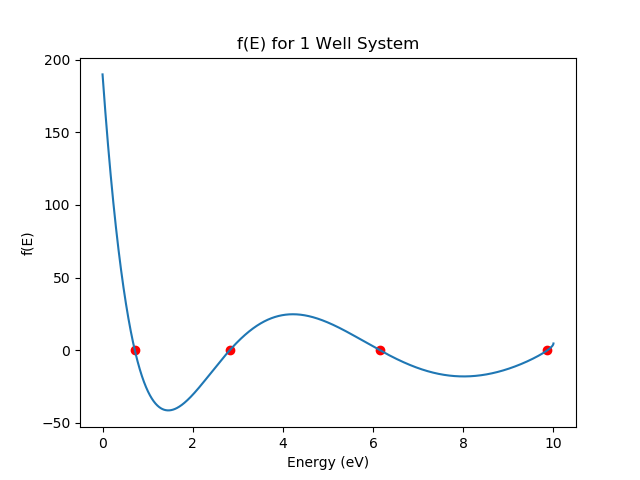
\includegraphics[width=.3\textwidth]{../figs/q2_19_1_well.png}
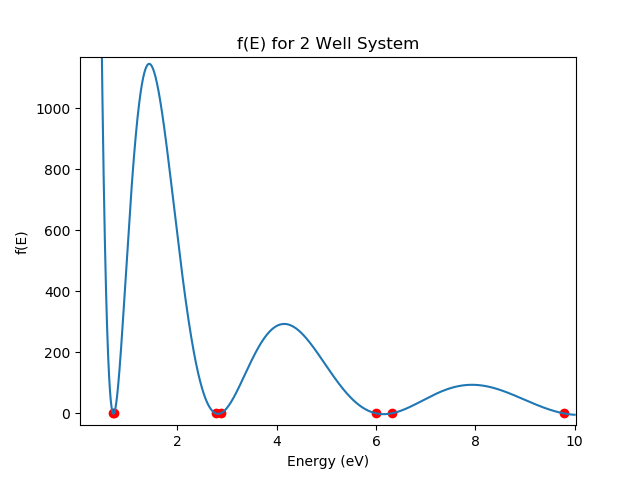
\includegraphics[width=.3\textwidth]{../figs/q2_19_2_well.png}
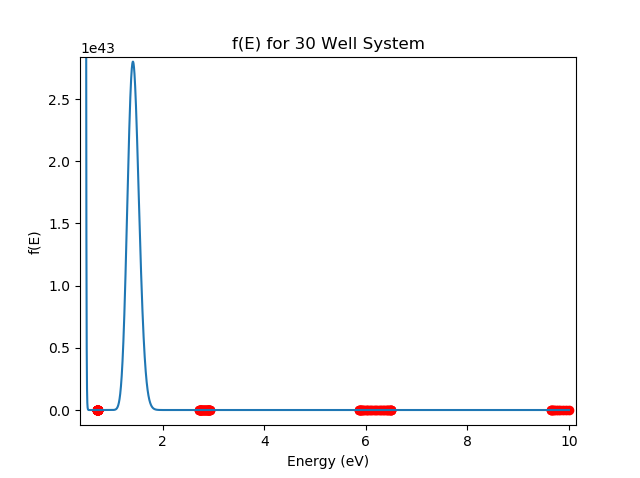
\includegraphics[width=.3\textwidth]{../figs/q2_19_30_well.png}
\end{center}
\captionof{figure}{$f(E)$ for 1, 2, and 30 well systems. We can see that even though the number of Energy eigenstates increase, they cluster at the same ranges at (0.7 eV, 2.8eV, 6.2 eV, and 9.8 eV) for this configuration.}
\vspace{1em}
\noindent When we zoom into the 6.2 eV range, we get the following plots:
\begin{center}
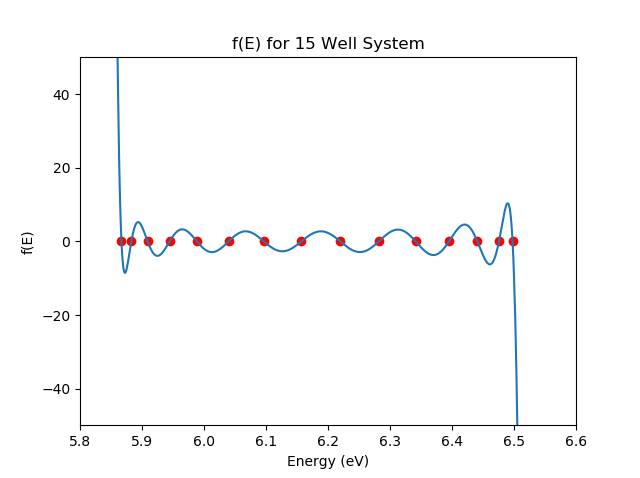
\includegraphics[width=.3\textwidth]{../figs/q2_19_15_well_zoom.png}
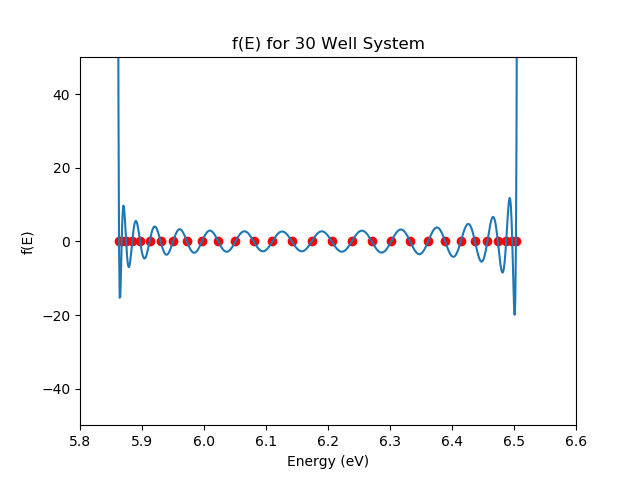
\includegraphics[width=.3\textwidth]{../figs/q2_19_30_well_zoom.png}
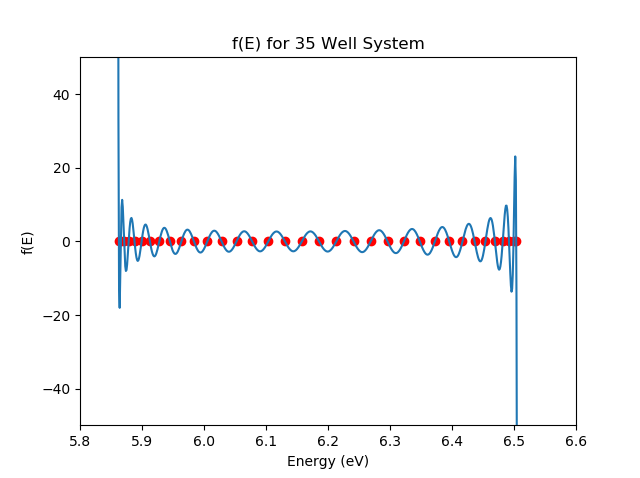
\includegraphics[width=.3\textwidth]{../figs/q2_19_35_well_zoom.png}
\end{center}
\captionof{figure}{$f(E)$ for 15, 30, and 35 well systems. The more we increase the number of wells, it seems that the energy levels are coupling and creating a fringing pattern remiinscent of energy splitting.}
\vspace{1em}
This makes sense. On their own, a single well has distint energy levels. We we couple two wells that are the same together, their potentials will overlap and, with the even and odd cases, will cause a splitting of the energy eigenstates. That is why there seems to be a broadening of our Energy eigenvalues.
\\ \\
\noindent However, this broadening can only go so far, as seen with the higher-order wells. As we add more and more wells, it is true that the enrgy eigenvalues increase as well, but they cluster in specific ranges. This is because the interactions of the wells will cause fine-splitting and not huge changes, so merely a pertubation. As we increase our number of wells to infinity, we will get finer and finer splittings, up until we can a continuous region where all values in that region is an energy eigenvalue. However, we will still have these distinct ranges of where we can find these energy eigenvalues.
\end{document}
